\subsection{Cross validation}
\label{se:cross_validation}
When constructing a regression model from a data set, over-fitting the data can be a problem. Including too many parameters and/or allowing too high order of the model would give a very good representation of the present roll damping data, but large extrapolation errors when the model is used on other data. K-fold cross validation has been used to ``mimic" this situation. The data has been split into five smaller sets (folds). Four of the folds are used to train the model and the fifth is used for testing (validation). The validation is done by calculating the coefficient of determination $R^2$ for the fitted model. This is done for all five possible train/test combinations. 
The folds are constructed in a random way with the restriction that all data for a particular ship should be in the same fold. Five folds are generated 20 times randomly, giving 100 values of $R^2$ from the train-test-procedure for each model. The mean values and standard deviation of these 100 values of $R^2$ are shown in Tab.(\ref{tab:crossvalidation}). The mean and standard deviation of $R^2$ for the SI-method in this table was calculated directly, instead of using cross validation, since it does not rely on the SSPA data.


\begin{table}[H]
    \centering
    \caption{Statistics from cross validations with all models}
   \begin{tabular}{lrr}
\toprule
{} &  \$mean(R\textasciicircum 2)\$ &  \$std(R\textasciicircum 2)\$ \\
model                      &              &             \\
\midrule
Simplified Ikeda           &         0.31 &             \\
Simplified Ikeda corrected &         0.59 &        0.16 \\
New regression             &         0.77 &        0.10 \\
\bottomrule
\end{tabular}

    \label{tab:crossvalidation}
\end{table}
    

%\begin{figure}[H]
%\vspace{-0.5cm}
%\centering
%  \centering
%  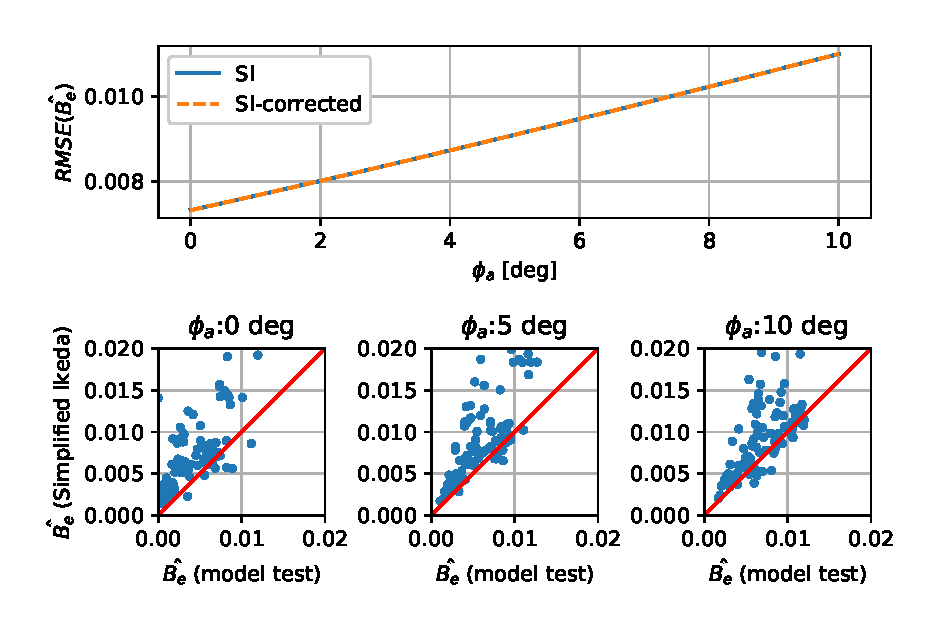
\includegraphics[]{figures/ikeda_corrected_phi_a.eps}
%  \vspace{-0.5cm}
%  \caption{Root mean square error of roll damping prediction between the SI-method, %corrected SI-method and the model test results (upper plot). Influence of roll %amplitude $\phi_a$ on $\hat{B_e}$ between the corrected SI-method and model tests for %$0^{\circ}$ (bottom left plot), $5^{\circ}$ (bottom middle plot) and $10^{\circ}$ %(bottom right plot), respectively.}
%  \label{fig:ikeda_phi_a_correction}
%\end{figure}
